\documentclass[a4paper,11pt,openany]{article}
\usepackage[utf8]{inputenc}
\usepackage[czech]{babel}
\usepackage{geometry}
\usepackage{tikz,multirow,listingsutf8,multicol,amsmath,amsfonts}
\lstset{language=python,showstringspaces=false,stringstyle=\color{orange},basicstyle=\ttfamily\large,keywordstyle=\color{blue!60!black}}
\geometry{left=20mm,right=20mm,top=20mm,bottom=20mm}
\parindent=0mm
\parskip=0mm
\usepackage{lipsum}
\newcommand{\quotefont}[2]{
	#1 [online]. [Citováno \today].\\
	Dostupné z:\\\small \ttfamily #2 \normalfont
}
\newcommand{\float}{\texttt{float}}

\begin{document}
\begin{center}
\pagenumbering{arabic}
{\huge \textbf{(a,b)-stromy}}\\\vspace{\baselineskip}Zápočtová práce z Programování I pro pokročilé\\
\vspace{10mm} {\large Jiří Škrobánek\footnote[1]{Matematicko-fyzikální fakulta Univerzity Karlovy, {\ttfamily jiri@skrobanek.cz}}}\\
\vspace{10mm}\today, Ostrava
\end{center}
	
\section*{Abstract}
	
This documentation describes the entire functionality of (a,b)-trees implementation in Python 3 by Jiří Škrobánek. Aside from listing all methods, principles of (a,b)-trees are explained and complexity of used algorithms is briefly analysed.
	
\tableofcontents
	
\section{Definice}
(a.b)-strom je strom. Musí platit $(a,b) \in \mathbb{N}^2, 2 \leq a, 2a - 1 \leq b $. (a,b)-strom je buďto prázdný, nebo mají všechny vnitřní vrcholy nejméně $a$ synů a nejvýše $b$ synů. Výjimkou je kořen, jenž musí mít mezi 2 a $b$ syny. Všechny listy leží v jedné hladiny. Vnějším vrcholům jsou přiřazeny unikátní klíče (prvky lineárně uspořádané množiny). Vnitřním vrcholům je přiřazen maximální klíč z jeho synů. Ve vnitřním vrcholu jsou uloženy klíče synů ve vzestupném pořadí. Pro každý podstrom platí, že mimo podstrom neexistují vnější vrcholy, které mají nižší klíč než maximální klíč v podstromu a zároveň vyšší klíč než minimální v~podstromu.
	
V tomto stromě se dá vyhledat vnější vrchol dle klíče v logaritmickém čase vzhledem k počtu vnějších vrcholů. Přidávání a odebírání listů rovněž funguje v logaritmickém čase.
	
Speciálním případem (a,b)-stromů pro $2a-1=b$ jsou B-stromy, mimo jiné oblíbený 2-3-strom.
	
\section{Metody}
Knihovna obsahuje třídy \texttt{InternalNode} a \texttt{ExternalNode} pro vnitřní a vnější vrcholy a třídu \texttt{ABTree}, která má metody popsané níže.
	
Počet vnějších vrcholů ve stromě značíme $E$.
	
\begin{lstlisting}[language=python,frame=none]
__init__(a: int,b: int)
\end{lstlisting}
Vytvoří (a,b)-strom pro konkrétní hodnoty $a,b$.
	
Výjimky: \texttt{ValueError}: Neplatná volba parametrů.
	
Složitost: $\mathcal{O}(1)$
\begin{lstlisting}[language=python,frame=none]
insert(self, key: int, value=None)
\end{lstlisting}
Vloží do stromu uspořádanou dvojici (key, value). Value může být libovolného typu nebo \texttt{None}.
	
Výjimky: \texttt{ValueError}: Strom již klíč obsahuje.
	
Složitost: $\Theta(\log(E))$
	
\begin{lstlisting}[language=python,frame=none]
delete(self, key: int)
\end{lstlisting}
Vymaže ze stromu vnější vrchol s klíčem \texttt{key}.
	
Výjimky: \texttt{ValueError}: Strom klíč neobsahuje.

Složitost: $\Theta(\log(E))$

\begin{lstlisting}[language=python,frame=none]
contains(self, key: int)
\end{lstlisting}
	
Vrací: \texttt{bool} Zda strom obsahuje daný klíč.

Složitost: $\Theta(\log(E))$
	
\begin{lstlisting}[language=python,frame=none]
find(self, key: int)
\end{lstlisting}
	
Vrací: Hodnotu ve vnějším vrcholu s daným klíčem.
	
Výjimky: \texttt{ValueError}: Strom klíč neobsahuje.
	
Složitost: $\Theta(\log(E))$
	
\begin{lstlisting}[language=python,frame=none]
item_count(self)
\end{lstlisting}
	
Vrací: \texttt{int} Počet vnějších vrcholů ve stromě.
	
Složitost: $\mathcal{O}(1)$
	
\begin{lstlisting}[language=python,frame=none]
find_leq(self, key: int)
\end{lstlisting}
	
Vrací: \texttt{(k, value)} Uspořádaná dvojice klíče a hodnoty z vnějšího vrcholu, který má maximální klíč v množině vrcholů s klíčem v intervalu $\left( -\infty, key\right\rangle $
	
Složitost: $\mathcal{O}(\log E)$
	
\begin{lstlisting}[language=python,frame=none]
find_lesser(self, key: int)
\end{lstlisting}
	
Vrací: \texttt{(k, value)} Uspořádaná dvojice klíče a hodnoty z vnějšího vrcholu, který má maximální klíč v množině vrcholů s klíčem v intervalu $\left( -\infty, key\right) $
	
Složitost: $\mathcal{O}(\log E)$
	
\begin{lstlisting}[language=python,frame=none]
find_geq(self, key: int)
\end{lstlisting}
	
Vrací: \texttt{(k, value)} Uspořádaná dvojice klíče a hodnoty z vnějšího vrcholu, který má minimální klíč v množině vrcholů s klíčem v intervalu $\left\langle key, \infty \right) $
	
Složitost: $\mathcal{O}(\log E)$
	
\begin{lstlisting}[language=python,frame=none]
find_greater(self, key: int)
\end{lstlisting}
	
Vrací: \texttt{(k, value)} Uspořádaná dvojice klíče a hodnoty z vnějšího vrcholu, který má minimální klíč v množině vrcholů s klíčem v intervalu $\left( key, \infty \right) $
	
Složitost: $\mathcal{O}(\log E)$

\section{Příkladové použití}
Na obrázku \ref{code} vidíme použití stromu. Na vyhledání pomocí klíče můžeme použít funkci \texttt{\_\_get\_item\_\_} a na zjištění počtu záznamů ve stromě \texttt{\_\_len\_\_}.


\begin{figure}[h]
\lstinputlisting[frame=single,basicstyle=\ttfamily\normalsize]{../demo.py}
\caption{Příkladový program}
\label{code}
\end{figure}

Na obrázku \ref{output} vidíme výstup získaný spuštěním příkladového programu.

\begin{figure}
\lstinputlisting[frame=single,basicstyle=\ttfamily\normalsize]{out.txt}
\caption{Výstup příkladového programu}
\label{output}
\end{figure}

\section{Stručný popis algoritmů}
	
\subsection{Vkládání}
	
Vkládáme \texttt{key, value}.  Pokud  je  strom  prázdný  vytvoříme  kořen,  který  bude  mít  nově  vkládaný záznam jako jednoho syna a vrchol s klíčem $\infty$ jako druhého syna. Začneme u kořene. Z vrcholu přejdeme na jeho syna, který má nejbližší vyšší klíč než \texttt{key}.

Po vložení zavoláme algoritmus vyvažování na otce nově vzniklého vnějšího vrcholu.
	
\subsection{Hledání}

Pokud hledáme podle klíče \texttt{key}, začneme v kořeni a sestupujeme na syny s nejbližším vyšším klíčem, nebo případně klíčem rovným \texttt{key}. Pokud nedojdeme do vnějšího vrcholu s hledaným klíčem, strom klíč neobsahuje.

\subsection{Mazání}

Pokud je třeba vrchol vymazat, nejdříve ho je třeba najít ve stromě a potom odstranit. Pokud byl navíc maximálním klíčem v některých vnitřních vrcholech, je třeba změnit v jeho předcích klíče na druhý nejvyšší vrchol v otci mazaného vrcholu (Takový musí existovat.)

Může být porušeno vyvážení stromu, proto je třeba zavolat vyvažování na bývalého otce smazaného vrcholu.
	
\subsection{Vyvažování}

Pokud jsme přidávali nebo mazali od posledního spuštění vyvažování pouze jeden vrchol, povolený počet synů ve vrcholech může být porušen o nejvýše 1.

Pokud ve stromě zůstal kořen a jeden vrchol ($\infty$), strom se stane prázdným.

Kontrolu stromu vždy začínáme v nějakém vrcholu. A může se vyvíjet několika způsoby:

\begin{itemize}
	\item
	Pokud je kontrolovaný vrchol kořen, který má jediného syna, odstraníme ho z grafu a jeho syn se stane novým kořenem. Ukončíme vyvažování.
	\item
	Pokud je kontrolovaný vrchol kořen a má více než $b$ synů, rozdělíme ho na dva a vytvoříme jim nového otce, který bude kořenem stromu. Ukončíme vyvažování.
	\item
	Pokud má kontrolovaný vrchol více než $b$ synů: Rozdělíme jej na dva, oba vrcholy získají nejméně $a$ synů, rozdělených podle velikosti. Tím mohl otec získat příliš mnoho synů, kontrolu pokračujeme na něm.
	\item
	Pokud má kontrolovaný vrchol méně než $a$ synů: Zkontrolujeme, zda se nemůže levý nebo pravý rozdělit o syny s tímto vrcholem, aby měly oba alespoň $a$ synů. Pokud toto nejde, sloučením s jedním z nich vznikne vrchol s povoleným počtem synů. Poté je potřeba pokračovat s kontrolou v otci, protože ztratil jednoho syna.
	\item
	Pokud je vše s vrcholem v pořádku, vyvažování ukončíme.
\end{itemize}

Výsledkem vyvažování je platný (a,b)-strom.

\begin{figure}
	\centering
	\includegraphics{pics/drawing.pdf}
	\caption{Příkladový (3,5)-strom}
\end{figure}

\section{Analýza složitosti}

\subsection{Minimální vyváženost stromu}

Pokud má strom $e$ vnějších vrcholů, strom má hloubku nejvýše $\lceil\log_a e\rceil + 1$.

Z definice musejí mít všechny vnitřní vrcholy nejméně $a$ synů, a proto počet vrcholů hloubky $h$ ve stromě je nejméně $a^h$.

\subsection{Paměťová složitost}

Strom s parametry $(a,b)$ a $e$ záznamy zabírá v paměti $\Theta(e)$. Neuvažujeme, kolik zabírají samotné údaje, které do stromu ukládáme, pouze strukturu stromu a klíče. Strom má nejvýše hloubku $\lceil\log_a e\rceil + 1$. Jeden vnitřní vrchol v sobě obsahuje klíče a ukazatele na nejvýše $b$ dalších vrcholů. 

Můžeme tedy provést horní odhad tak, že všechny hladiny budou plné a bude jich teoretický maximální počet. V tomto případě je počet vnějších vrcholů roven $a$. Další úroveň obsahuje ve vrcholech klíče a ukazatele na externí vrcholy, ale všechny další obsahují nejméně $a$-krát méně klíčů, je jich $a$-krát méně. Součet takovéto geometrické řady je vždy pouze konstantním násobkem prvního členu, tedy $e$.

\subsection{Rychlost vyhledávání}

Vyhledávání se použije nejen v případě, že je potřeba získat z pole záznam, ale také při vkládání a odstraňování, je tedy nutné, aby probíhalo rychle. 

Jak plyne z algoritmu, začíná se ve stromě a sestupuje se až na spodní hladinu. V každém prošlém vrcholu se přitom porovná až $b$ klíčů. Pokud je hledání nakonec neúspěšné, proces se liší až posledním krokem.

Dohromady to dává $ \Theta(b\log_a e) $ operací ve stromě s $e$ záznamy.

\subsection{Rychlost vyvažování}

Vyvažování spouštíme na nějakém konkrétním vrcholu, pouze pro tento vrchol hrozí porušení počtu synů. Provádí se de facto dvě operace:

\textbf{Slučování} Pokud se uskuteční sloučení vrcholu, vrchol vzniklý po sloučení bude mít počet synů v pořádku. Jen jeho otce bude třeba preventivně zkusit vyvážit (pokud existuje). Nově vzniklý vrchol už je ale vyvážený a nebude se k němu potřeba vracet.

Hledání vrcholů ke sloučení i vyrábění nového vrcholu je práce s $ \mathcal{O}(b) $ klíči.

\textbf{Rozdělování} Vrcholy vzniklé rozdělením mají správný počet synů, vyvažování pokračuje otcem těchto vrcholů.

Protože máme již určeno jaká je maximální hloubka stromu a vyvažuje se maximálně 1 vrchol v každé hloubce, můžeme říci, že během vyvažování proběhne $ \mathcal{O}(e) $ operací.

\listoffigures
\begin{thebibliography}{10}
	\bibitem{aocp}
	KNUTH, Donald Ervin. The Art of Computer Programming. Upper Saddle River, NJ: Addison-Wesley, 2011. ISBN 978-0321751041.
\end{thebibliography}
\end{document}